\documentclass{beamer}

\usepackage{graphicx}
\usepackage{minted}
\usetheme{Frankfurt}

\title{Introduction to python}
\author{Jadavpur University Code Club}
\titlegraphic{
\includegraphics[width=.5\textwidth]{./img/python_o_1269231.jpg}}
\date{}

\begin{document}

\maketitle

\begin{frame}[fragile]{The hello world program}

	\begin{minted}{python}
		print("hello world")
	\end{minted}

	\pause

	\begin{center}
		
\includegraphics[width=.3\textwidth]{./img/images.jpg}
	\end{center}

\end{frame}

\begin{frame}[fragile]{Running the code}
	\Large{Two ways to do it:}
	\begin{itemize}
		\item Interactive mode
		\item Shell mode
	\end{itemize}
\end{frame}

\begin{frame}[fragile]{Variables}
	\begin{minted}{python}
		x = 1.0
		y = "hello world"
	\end{minted}
	\begin{center}
		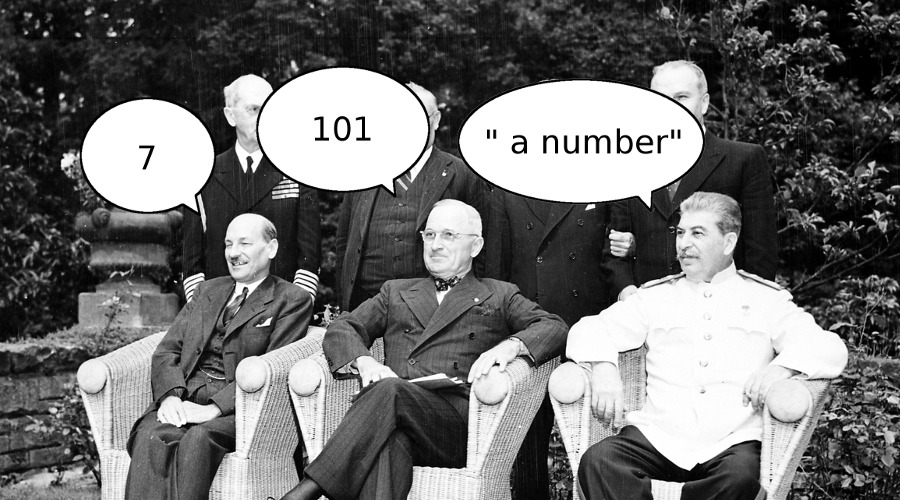
\includegraphics[width=.7\textwidth]{./img/variables.jpg}
	\end{center}
\end{frame}

\begin{frame}[fragile]{Indentation is important}

\begin{minted}{python}
	if foo:
	  if abc(x):
	    print(x)
	else:
	  print(y)
\end{minted}


\end{frame}

\end{document}
